\problemname{Orm}
\noindent

Igår vann lilla Olle det kända spelet \textit{Orm} för första gången. I Orm finns det ett $3 \times N$ stort rutnät. 
Spelaren kontrollerar en orm som består av ett antal segment. Till en början består ormen av ett enda segment, vilket vi
kallar för dess huvud. Varje sekund kan huvudet röra sig upp, ner, höger eller vänster. Om huvudet krockar med ett annat segment
så förlorar du spelet. Efter att huvudet rör sig, så förlorar ormen segmentet längst bort från huvudet (det äldsta segmentet som
tillhör ormen). Med andra ord kan man
föreställa sig att ormens kropp förflyttat sig en ruta. Under spelets gång kommer det att dyka upp äpplen på vissa rutor.
Om ormens huvud åker på ett äpple så försvinner äpplet, men segmentet längst bort från huvudet försvinner inte. Med andra ord
ökar ormens längd med $1$.

Om ormen fyller upp hela rutnätet har man vunnit spelet, eftersom man inte längre kan göra ormen längre. När Olle vill skryta för
sina vänner att han äntligen vunnit Orm, så tror de honom inte. För att övertyga sina kompisar tänker Olle rita upp hur hans Orm
såg ut när han vann. Tyvärr kommer han inte ihåg exakt hur den såg ut. Han kommer dock ihåg hur långt vissa rutor befann sig från
svansen (segmentet längst bort från huvudet). Givet en del av dessa avstånd, kan du hitta hur Olles orm såg ut?

\begin{centering}
  \begin{figure}[h]
      \centering
      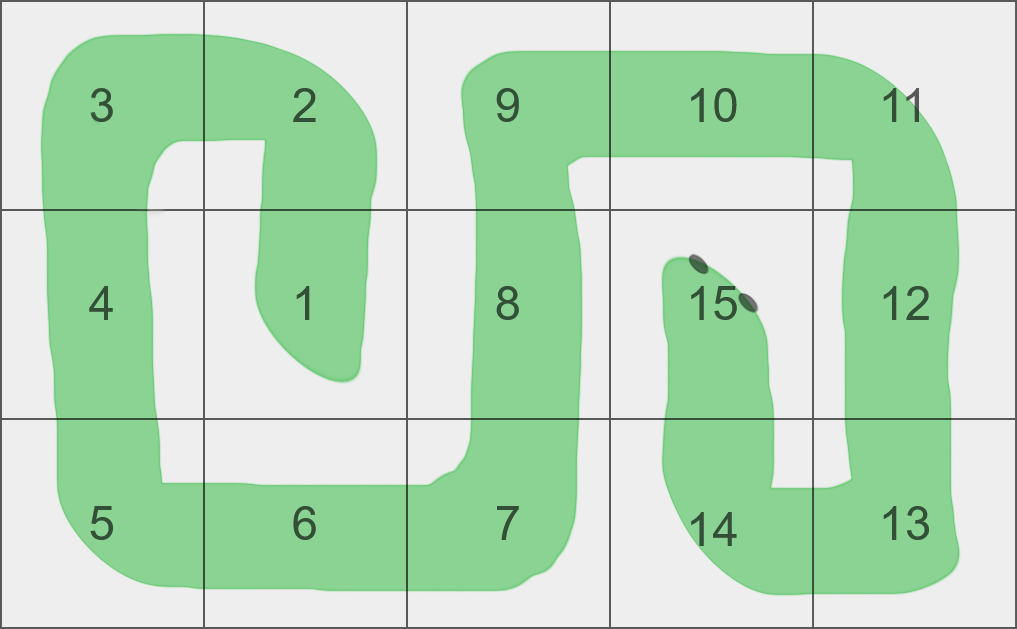
\includegraphics[width=0.8\textwidth]{snake.png}
      \caption{Bilden visar ett möjligt sätt som ormen kan se ut i exempelfall 1.}
  \end{figure}
\end{centering}

\section*{Indata}
Den första raden innehåller heltalet $N$ ($1 \leq N \leq 1000$), antalet kolumner i rutnätet.

Därefter följer tre rader som vardera beskriver en rad av rutnätet. Den $i$:te raden innehåller heltalen
$c_1, c_2, \dots, c_N$ ($0 \leq c_j \leq c_N$), avståndet mellan svansen och ormens kroppssegment på rad $i$ och kolumn $j$.
Om $c_j$ är $0$ betyder det att Olle glömde vad $c_j$ är. Alla $c_j$ som inte är $0$ är parvis unika. Det är även garanterat att det
finns minst en giltig lösning.

\section*{Utdata}
Skriv ut $3$ rader med $N$ heltal vardera, som beskriver en giltig vinnande orm. Varje heltal mellan $1$ och $N \cdot 3$
måste förekomma exakt en gång. För varje $i$ mellan $1$ och $N \cdot 3 - 1$ måste segmentet med tal $i$ ligga ovanför, nedanför,
till vänster eller höger relativt segmentet med tal $i+1$.

\section*{Poängsättning}
Din lösning kommer att testas på en mängd testfallsgrupper.
För att få poäng för en grupp så måste du klara alla testfall i gruppen.

\noindent
\begin{tabular}{| l | l | p{12cm} |}
  \hline
  \textbf{Grupp} & \textbf{Poäng} & \textbf{Gränser} \\ \hline
  $1$    & $15$         & $N \leq 10$  \\ \hline
  $2$    & $25$         & $N \leq 40$ \\ \hline
  $3$    & $30$         & $N \leq 300$ \\ \hline
  $4$    & $30$         & Inga ytterligare begränsningar. \\ \hline
\end{tabular}

